\documentclass[a4paper,12pt]{article}

\usepackage[utf8]{inputenc}
\usepackage{parskip}
\usepackage[ngerman]{babel}
\usepackage{graphicx}

\title{OOAD Übungsblatt 2}
\author{Dominik Tödling, Lukas Neuhold, Christoph Huber,\\ Stefan Mitterrutzner, Emanuel Moser}

\begin{document}
\maketitle
\part*{Abgabe 1}
\begin{center}
	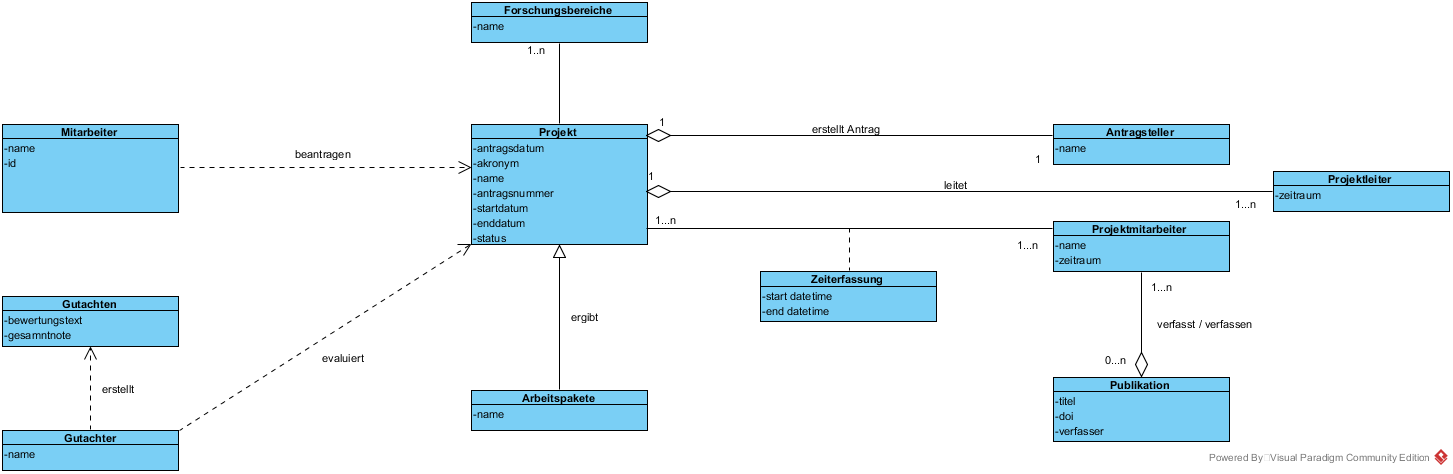
\includegraphics[scale=.57,angle=90]{Abgabe1.png}
\end{center}
\part*{Abgabe 2}
\section*{Business Case}
\begin{itemize}
	\item Viel einfachere Organisation von Timeslots/Räumen
	\item Alle immer auf dem gleichen Stand
	\item Automatische und individuelle Zeitplangenerierung
	\item Weniger administrativer Aufwand
\end{itemize}
\section*{Use Cases}
	\subsection*{Priorisierung und Szenarien}
	\begin{tabular}{|p{3cm}|c|p{3cm}|c|p{3cm}|c|}
		\hline
		\textbf{Student} & \textbf{Score} & \textbf{Lehrender} & \textbf{Score} & \textbf{Admin} & \textbf{Score} \\ \hline
		Anmelden & 10 & Anmelden & 10 & Anmelden & 10 \\ \hline
		Für Veranstaltung registrieren & 10 & Für Veranstaltung registrieren & 10 & Account erstellen & 10 \\ \hline
		Account erstellen & 10 & Account erstellen & 10 & Accounts authorisieren & 10 \\ \hline
		Kalender einsehen & 9 & Veranstaltung erstellen & 10 & Zeitpräferenzen eingeben & 8 \\ \hline
		Event erstellen & 3 & Kurs erstellen & 10 & Zeitplan verändern & 7 \\ \hline
		&& Kalender einsehen & 9 & Zeitplan überprüfen & 7 \\ \hline
		&& Prüfung erstellen & 9 & Veranstaltung erstellen & 5 \\ \hline
		&& Zeitpräferenzen eingeben & 8 & Kurs erstellen & 4 \\ \hline
		&& Event erstellen & 3 & Prüfung erstellen & 4 \\ \hline
		&&&& Für Veranstaltung registrieren & 3 \\ \hline
		&&&& Kalender einsehen & 3 \\ \hline
		&&&& Event erstellen & 3 \\ \hline
	\end{tabular}
	\newpage
	\subsubsection*{Anmelden}
		Klick auf “Anmelden” \\
		Anmeldefenster anzeigen \\
		User gibt Daten ein \\
		Überprüfe Daten \\
		User anmelden
	\subsubsection*{Account erstellen}
		Klick auf “Account erstellen” \\
		Registrierungsfenster anzeigen \\
		User gibt Daten ein\\
		Daten überprüfen und speichern\\
		User bestätigung anzeigen
	\subsubsection*{Für Veranstaltung registrieren}
		Klick auf “Für Veranstaltungen registrieren”\\
		User wählt Veranstaltung\\
		Registriere User für Veranstaltung\\
		Evtl. bei Zeitkollisionen Warning ausgeben\\
	\subsubsection*{Kalender einsehen}
		Klick auf “Kalender”\\
		Aus assoziierten Veranstaltung (registriert/hält ab) Kalender generieren und anzeigen
	\subsubsection*{Veranstaltung erstellen}
		Klick auf “Veranstaltung erstellen”\\
		User wählt Art der Veranstaltung, Dauer, Namen, etc. und evtl Zeit-/Raumpräferenzen\\
		Veranstaltung erstellen und in geeignetem Zeitslot und Raum eintragen\\
		Evtl Warning ausgeben wenn außerhalb der eingegebenen Präferenzen
	\subsection*{Use Case Diagramm}
	\begin{center}
		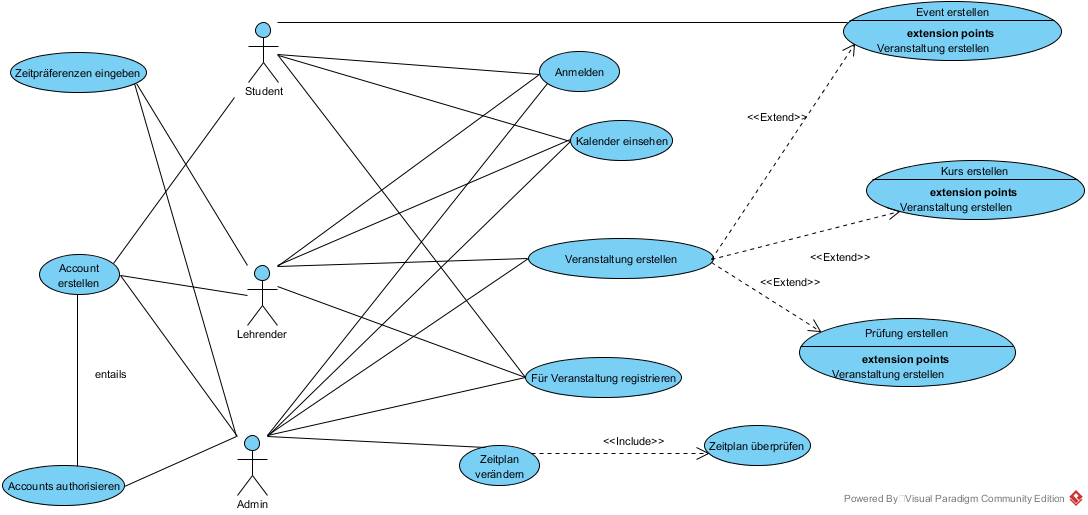
\includegraphics[scale=.5]{UseCaseDiagram.png}
	\end{center}
\section*{UML Analyse-Klassendiagramm}
\begin{center}
	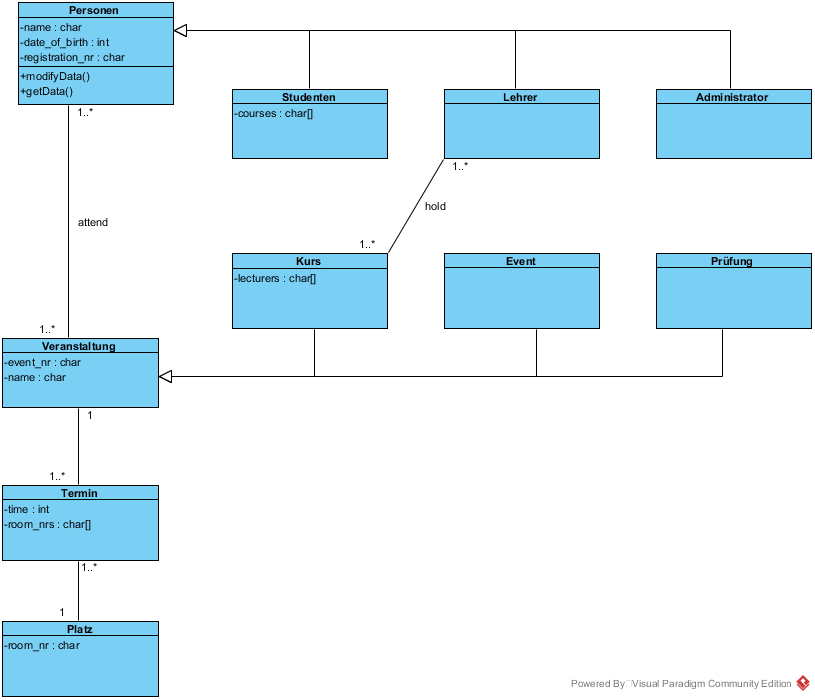
\includegraphics[scale=.5]{ClassDiagram.png}
\end{center}
\section*{Projektplan}
\begin{enumerate}
	\item Datenbankarchitektur
	\item Veranstaltungen erstellen/besuchen
	\item Zeitplan einsehen
	\item Automatische Zeitplanung/Constraints
	\item Account Erstellung/Anmeldung
	\item Verschiedene Arten von Users mit verschiedenen Berechtigungen
	\item Zeitpräferänzen für Vortragende
	\item Semestersystem
	\item Endgültige Daten Einfügen
\end{enumerate}
Deadlines noch offen.
\section*{Screenshots}
	\begin{center}
		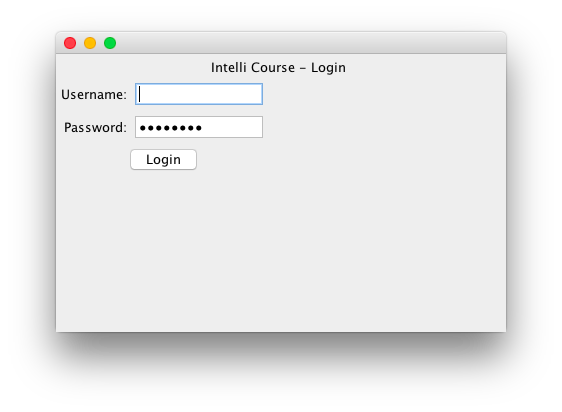
\includegraphics[scale=.5]{Login.png}
		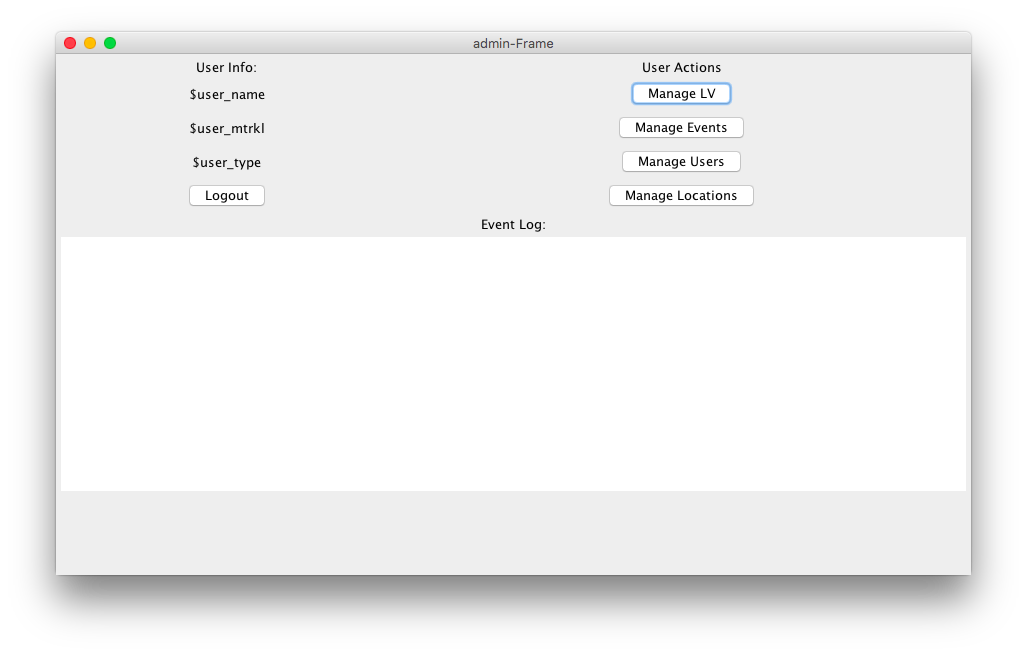
\includegraphics[scale=.4]{Admin.png}
		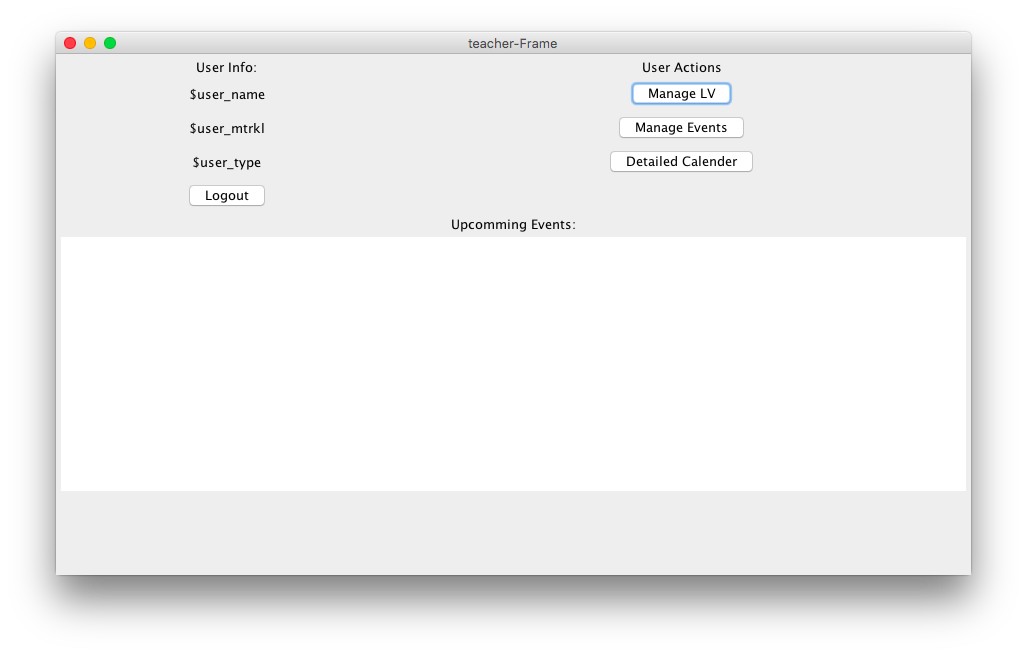
\includegraphics[scale=.4]{Teacher.png}
		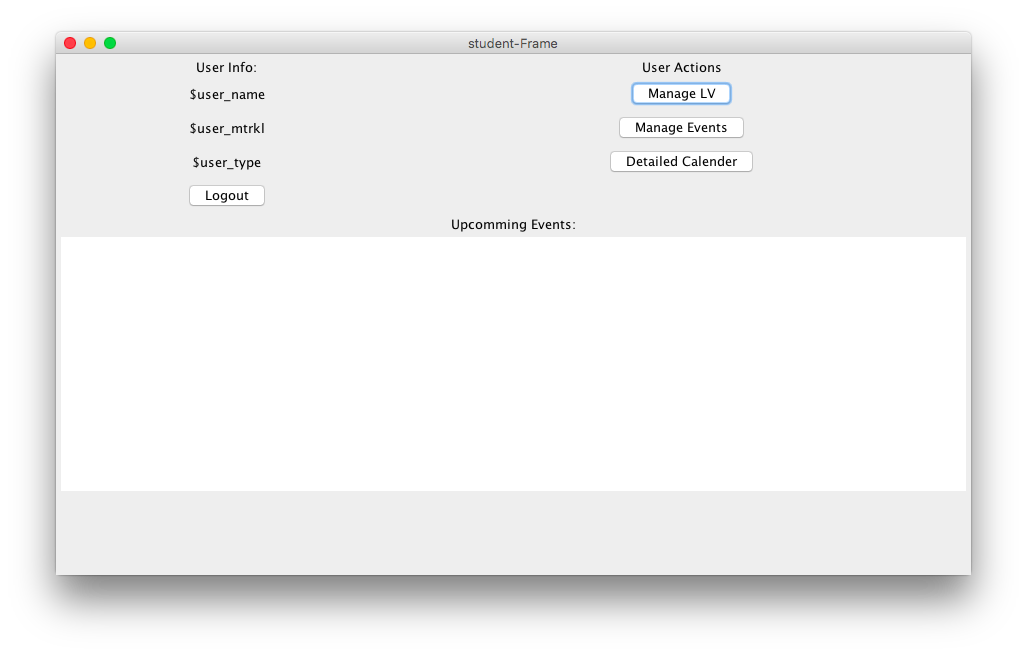
\includegraphics[scale=.4]{Student.png}
		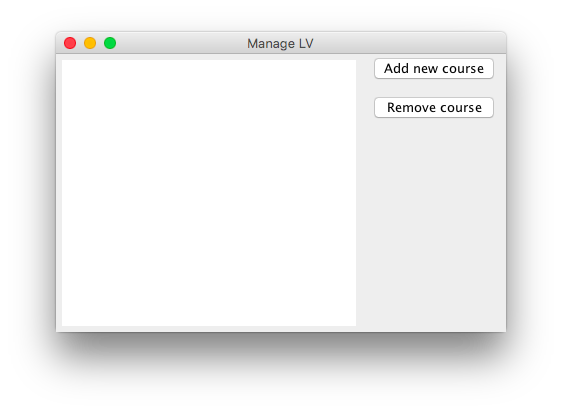
\includegraphics[scale=.6]{ManageLV.png}
		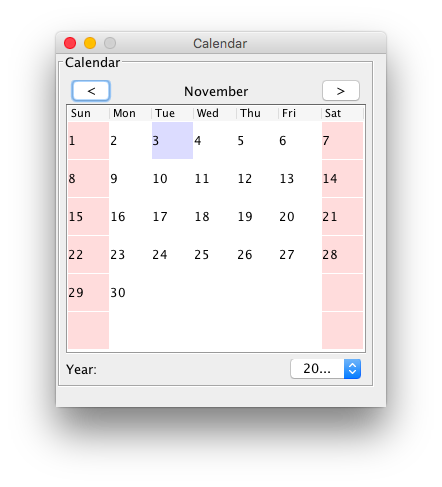
\includegraphics[scale=.6]{Calendar.png}
	\end{center}
\end{document}